%1. La memoria incluirá una portada portada normalizada con la siguiente información: título en castellano, título en inglés, autores, profesor director, codirector si es el caso, curso académico e identificación de la asignatura (Trabajo de fin de grado del Grado en - nombre del grado correspondiente-, Facultad de Informática, Universidad Complutense de Madrid). Los datos referentes al título y director (y codirector en su caso) deben corresponder a los publicados en web de TFG, según lo indicado en el punto 6 de la sección III de esta normativa. 
% 2. en cada apartado
% 3. La memoria constará de un mínimo de 25 páginas para los proyectos realizados por unúnico estudiant

\documentclass[12pt, a4paper, hidelinks]{article}
\usepackage[spanish, english]{babel} 	% language
\usepackage{tocloft}					% table of contents

% for sections
\renewcommand{\cftsecleader}{\cftdotfill{\cftdotsep}} 

% images
\usepackage{graphicx}
\graphicspath{ {./images/} }

% wrap around images
\usepackage{wrapfig}

% tables
\usepackage{longtable}
\usepackage{booktabs} 	% line separators

%links
\usepackage{hyperref}
\hypersetup{
	colorlinks=false
}

% text columns
\usepackage{multicol}
\setlength{\columnsep}{1cm}


\title{\textbf{Sampler plugin for digital audio workstations}}

%\title{\textbf{Sampler plugin for digital audio workstations\\---\\ Instrumento virtual basado en samples para estaciones de trabajo de audio digital}}

%\author{Juan Chozas Sumbera}
\date{\vspace{-10ex}}

\begin{document}
	\maketitle
	\begin{center}
		\textbf{Trabajo de Fin de Grado en Ingeniería Informática}\\
		
		~\newline
		\textbf{\large{Juan Chozas Sumbera}}
		
		~\newline
		Dirigido por
		
		\textbf{Jaime Sánchez Hernández\\
		Miguel Gómez-Zamalloa Gil}
		
		
		~\newline
		
\includegraphics[width=0.5\textwidth]{logo_UCM.png}\\
		~\newline
		
		\textbf{\large{UNIVERSIDAD COMPLUTENSE DE MADRID}}\\
		
		\textbf{FACULTAD DE INFORMÁTICA}
	\end{center}

	
	
	% 2. La memoria debe incluir la descripción detallada de la propuesta hardware/software realizada y ha de contener: 
	% a. un índice, 
	% \tableofcontents % despues del resumen y antes de la intro
	\newpage

	
	% b. un resumen y una lista de no más de 10 palabras clave para su búsqueda bibliográfica, ambos en castellano e inglés, 
	\newpage
	\huge
	\textbf{Abstract}\\

	\normalsize
	Music production is at anyone's reach. Nowadays, computers, smartphones and tablets are able to run software that provides the necessary tools to compose music. Digital Audio Workstations (DAWs) are found at the more sophisticated end of the spectrum. These feature-packed programs are the type that you would find in locations ranging from the aspiring musician's personal computer to the most professional recording studio in your city. One of the most powerful characteristics of these environments is being extensible via plugins. \par	
	The sampling techniques that emerged during the end of the 20th century gifted the world with new methods of music composition. The technique that this project develops upon consists in the creation of an instrument using audio recordings as its only source of sound. The nature of the process is far from complex and it can be streamlined to provide a fast way to design a bespoke instrument. By implementing this tool as a plugin, the instrument takes the form of a loadable module that is readily accessible to anybody working on a DAW.
	
	\vspace*{\fill}
	\large
	\textbf{Key words}\\
	
	\vspace{-1em}
	\normalsize	
	\noindent music, sound, sampler, sampling, instrument, MIDI, DAW, plugin, VST, synthesizer\\

	\newpage
	\huge
	\textbf{Resumen}\\
	
	\normalsize
	Cualquier persona tiene a su alcance la producción musical. El mundo en el que vivimos esta plagado de dispositivos capaces de ejecutar programas que ofrecen todas las herramientas necesarias para componer música.	Las estaciones de audio digital son los programas que ofrecen la mayor gama de herramientas para la creación de música. Es el tipo de software que no puede faltar en los ordenadores de los músicos principiantes ni de los estudios de grabación más sofisticados. Estos entornos pueden ser enriquecidos mediante módulos externos (plugins), extendiendo la gama de utilidades que pone a disposición del usuario.\par
	A finales del siglo 20 emergieron nuevas técnicas de muestreo, nuevas maneras de producir música utilizando grabaciones de sonido. Este proyecto utiliza estas técnicas de base para ofrecer una manera rápida de crear un instrumento a medida que utiliza regiones de una muestra para producir sonido. El proceso es sencillo por naturaleza y se puede implementar de forma eficiente para hacer un proceso sin demoras innecesarias del diseño de un instrumento basado en muestras. La implementación en forma de plugin hace que el instrumento sea accesible para todo el que trabaje con una estación de audio digital.

	
	\vspace*{\fill}
	\large
	\textbf{Palabras clave}\\
	
	\vspace{-1em}
	\normalsize	
	\noindent música, sonido, muestra, muestreo, instrumento, MIDI, DAW, plugin, VST, sintetizador
	
	
	
	\newpage
	% a. un índice, 
	\tableofcontents


	% c. (25 pg entre c y d) una introducción con los antecedentes, objetivos y plan de trabajo, 
	\newpage
	\section{Introduction}
	\subsection{Background}
	The technique of sampling dates back to the 1960s when recordings were captured on tape. Thanks to a hardware design that made contact between the playback head and different sections of a moving tape, musicians could play the distinct recordings on keyboards of instruments such as the Mellotron. During the 1980s, the popularity of drum machines increased significantly. Many drum machines were sample-based, i.e. they created sounds using digitally stored samples, whereas the alternative was to synthesize sound in an analog fashion. In 1988, the first Music Production Center (MPC) by Akai was made available to the public: a sample-based music workstation that was capable of arranging samples of all lengths in its sequencer to produce full fledged music tracks without the need for additional instruments or hardware. In a recipe for music, an MPC could be the only ingredient, reaching a vast number of musicians because of its affordability in comparison to previous means of music production. It is a tool that gave artists a new way to create music, a technique that has been a foundation to several genres and highly influential to music as a whole.\par
 	
 	In a world of highly complex information systems, digital music production has been developed thoroughly. When it comes to modern music composition, Musical Instrument Digital Interface (MIDI from now on) protocols provide grounds for an alternative to \textit{analog} instruments. This standard erects a bridge for communication between digital instruments and computers, providing the world of digital music production with the tangible interfaces of normal instruments. The MIDI standard provides, among many other features, a communications protocol that encodes music events. This manifests in the form of messages which describe data such as the pressing, releasing, and velocity of musical notes. 	

 		\begin{longtable}[]{@{}cc@{}}
 			Syllabic & Alphabetical \tabularnewline
 			\midrule
 			Do  & C \tabularnewline
 			Re  & D \tabularnewline
 			Mi  & E \tabularnewline
 			Fa  & F \tabularnewline
 			Sol & G \tabularnewline
 			La  & A \tabularnewline
 			Si  & B \tabularnewline
 			\caption{Musical notes in syllabic and alphabetical form}
 			\label{table:notes}
 		\end{longtable}
 	A digital audio workstation (DAW from here on out) is a software environment for music production. These workstations revolve around MIDI, which provides an encoded language for musical notes. See Table \ref{table:notes} for a table of the syllabic and alphabetical equivalents of musical notes. 
 	\par
 	
	One can have an extensive range of digital synthesizers, samplers, and effect chains all working simultaneously in a DAW, the type of software that provides a playground that routes audio between racks of components and effects, making music production a possibility to anyone that owns a computer. DAWs have an element called a sequencer, which serves as a sort of digital equivalent to sheet music. The sequencer is where a musician draws out the music, placing small rectangles on a grid to represent the notes, their length, and their duration. These arrangements are made for instruments such as synthesizers or samplers to trigger the sounds they produce, and can be auto generated, drawn out manually, or recorded in real time with a MIDI controller. Auto generated patterns consist of filling a set length of time with notes separated by constant intervals, so as to mimic the timing of a metronome, for example. Patterns that are recorded in real time are made with the DAWs recording function, which is activated to record MIDI events from a controller. A user may have an instrument loaded during this recording period, so the user can know what sounds are being produced. It is important to highlight that it is a sequence of MIDI events that is recorded by the DAW, not the actual sounds being produced by the instrument. The relevant events associated to this process are: note-on events, the signal that a note has been pressed; note-off events, the signal that a note has been released. A musical note is associated to note-on and note-off events, having the note and octave being encoded as an integer in the range of $[0, 127)$. In addition, associated to note-on events is an element called velocity, which is a measure of the intensity of the note. The velocity of a note is sometimes processed by instruments to generate softer or stronger sounds. Some samplers use note velocity to trigger a sample from a set, i.e. a lower intensity recording of a snare drum for lower velocities as opposed to a sample of a powerful snare drum hit when the velocity is a higher range.
 	\par
 	
	DAWs can be extended with plugins in the form of effects or instruments. The former normally have a sound-based input-output relation with the DAW, meanwhile instruments will take MIDI messages and produce a sound as an output. For example, a simple plugin could be a sine wave based instrument. The wave's frequency will depend on the key being pressed, and the force applied to the key will dictate the amplitude of the wave. This plugin, although simple, could be considered a synthesizer. A sampler is a synthesizer that uses samples rather than oscillators to produce sound.  The sources of the sounds it produces are samples, which can be described as clips of audio that are stored in a digital format within the sampler's memory. You're likely to find that hardware and software samplers offer sets of "stock" samples that are loaded by default. The option to load samples from an external source such as an SD card is also common, just like recording external input from a recording device such as a microphone. As is the case with non sample based synthesizers, there are several ways that the samples can be manipulated. This sampler, in particular, takes the form of a plugin for digital audio workstations. Once samples are loaded, the user associates the samples to MIDI notes to enable pattern arrangements and playback on controllers. The DAW then routes MIDI messages describing the notes being played into the plugin, which in turn processes the input to produce a stream of audio that is returned to the host as sound. The sound produced by this sampler comes from sub-samples: designated regions of a main sample. Once assigned to MIDI notes, these regions will then be playable from MIDI controllers. The DAW will also be able to trigger the sub-samples from an arrangement of notes in a pattern made for the sampler.\par 
	
	To explore the ways in which a sampler can manipulate sound, I will start with \textit{envelopes}, which dictate the way a sound changes over time. Envelopes affect playback every time it is triggered, and are commonly composed of four parameters. 	
	\begin{wrapfigure}[12]{r!}{188pt}
		\centering
		\vspace{-33pt}
		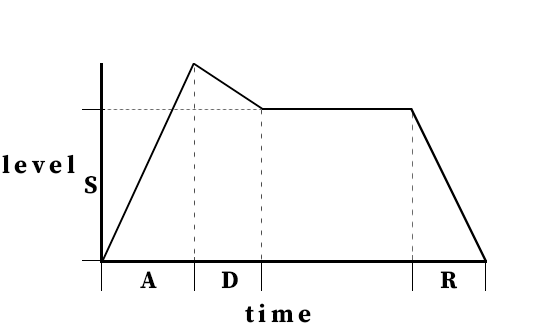
\includegraphics[scale=0.4]{envelope.png}
		\caption{ADSR parameters in envelopes}
		\label{fig:envelope}
	\end{wrapfigure}
	The first one  comes into play upon note-on events, i.e. on a key press: \textit{attack}, describing the time it takes for the sound's level to rise from zero to its peak. Next, \textit{sustain} is the level at which the sound will hold until a note-off event, i.e. when a key is released. \textit{Decay} depends on sustain, and it describes the time it will take for the level to go from peak to sustain. Finally, \textit{release} is the tail end of the envelope. Starting on note-off events, it describes the time it will take to reach zero level from sustain level. These four concepts form the acronym ADSR, and can be pictured as a plot of level against time in Figure \ref{fig:envelope}. You may have noticed that three of the parameters refer to a time measure, whereas sustain refers to a level. \par 
	
	Some other ways to manipulate sounds are by altering volume and panning. Volume refers to the level of the sound, whereas panning dictates the direction the sound is perceived to be coming from. Panning only applies to stereo systems, where there the output is composed of two channels that represent left and right. 
	
	
	\newpage
	\subsection{Objectives}
	Most DAWs have built in samplers or similar tools that allow a user to sample sound and directly manipulate it so as to employ sampling techniques. In most cases, these tools are more than capable of providing the means to translate these techniques into action, however, depending on the DAW, you may be hindered due to the program's presentation. Whether it be the user interface, the imposed workflow, or the minimum amount of steps required to reach your sampling goals, it is likely that the process involves inconveniences.\par 
	Personally, I find that there are a minimum of three steps to achieve a usable sampler configuration. First, a main sample must be loaded. Second, the process of \textit{chopping} the sample, where a set of subsections are created within the sample, creating sub-samples otherwise known as \textit{chops}. Third comes the assignment of chops to MIDI notes, in other words, the mapping of sample subsection playback to a controller's keys. These steps are a prerequisite to playing chops on the controller. At this stage, the user can experience the instrument and judge whether it is necessary to take a step back and make adjustments, for example, shifting the start time of a chop, creating/deleting a chop, or moving the trigger note to another of higher convenience. All of this implies that the design of a sampler instrument is an iterative process, and that the user may keep reforming it in several ways to fit the necessities of the creative process in musical composition.
	\par	
	The aim here is to reduce the amount of user interaction required to translate an idea into sound. For the simple implications of sampling techniques, the means by which you achieve a minimum setup with which you can play around and manifest ideas should be straightforward. With this project the intention is to strip the process of whatever element that is not essential to it. By downsizing in the features that a DAW would offer, I aspire to build a plugin strictly optimized for sampling. %This means that the user will be able to load, chop, and play samples with speed and ease in a reduced sequence of actions. In addition, the user should also be able to make fast corrections and tweaks to further develop the instrument. 
	\par
	The capabilities of the sampler can be summarized to four key functionalities:
	\begin{itemize}
		\item Capacity to load an audio clip as the main sample 					% TODO MORE THAN ONE SAMPLE?
		\item Manual chopping and automatic chopping with peak detection algorithm 	% TODO link aubio
		\item Visual representation and audio preview of the main sample and its chops
		\item Editable envelope parameters for each chop							% TODO chop pan? vol? filters?
	\end{itemize}
	
	% d. (25 pg entre c y d) resultados y discusión crítica y razonada de los mismos, con sus conclusiones,
	\newpage
	\section{Results}
	%intro juce, support for plugins, extensive tutorials and examples
	To implement the sampler, I used the JUCE application framework. It has cross-platform support is fully implemented in C++. 
	

	
	
	\subsection{Conclusion}
	 
	\newpage
	% e. bibliografía.
	\section{Bibliography}
	
\end{document}